\chapter{Technical Description}\label{ch:technical_description}
Quantum computing can help machine learning in two ways- data and computation. Based on this Quantum Machine Learning can be divided into 3 approaches.
\begin{enumerate}
\item Quantum enhanced Machine Learning ( classical data with quantum algorithms) 
\item Classical learning applied to quantum systems ( classical algorithm with quantum data)
\item Fully quantum machine learning (both data and algorithm is quantum based)
\end{enumerate}
\begin{figure}[H]
\centering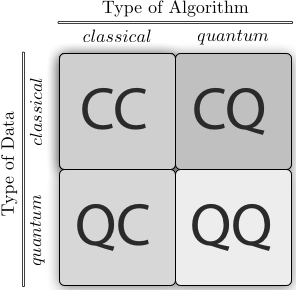
\includegraphics[width=.3\textwidth]{images/approach.png}
\caption{Approaches in Quantum Machine Learning}
\end{figure}
\section{Quantum Enhanced Machine Learning}
Quantum Enhanced Machine Learning is the most promising of these methods on early quantum computers. Such algorithms typically require one to encode the given classical dataset into a quantum computer so as to make it accessible for quantum information processing. Machine learning techniques use mathematical algorithms and tools to search for patterns in data. The most important and time taking parts of machine learning algorithms are searching, sampling and optimization. We explain how these can be improved by Quantum Computing in the following sections.
\subsection{Search: Grover's algorithm}
When you compute Grover's Algorithm you are simultaneously testing every input value to see which is the correct input value. Using quantum superposition you can get qubits in a state that represents all possible inputs. Then run that superposition of states through some function to get each input together with its associated output. You are given a list of $n$ elements, and you know that one element satisfies a certain condition, while the other n-1 elements don't. Basically, this is an algorithm for finding a specific element in an unordered list. A classical computer would not be able to exploit any structure in this problem and therefore needs to scan up to $n-1$ elements to find the one needed.
Prepare $n$ qubits in a uniform state so that all $2^n$ numbers are in a uniform superposition, each with a coefficient of $1/\sqrt{n}$ If we would measure the $n$ qubits now, all $2^n$ results would be equally likely.\\
Then run the Grover iteration $k$ times, which consists of two steps (which can be merged into 1 step):
\begin{enumerate}
\item Negate the coefficient of the sought element. This is a unitary operation, which leaves all elements not satisfying the condition as they are and only negates the intended one.
\item Reflect all quantum states at the arithmetic mean of all quantum states. This also is a unitary operation.
\end{enumerate}
Each iteration amplifies the coefficient of the correct solution while damping the coefficient of all $n-1$ incorrect solutions, however only to a certain point.
If you choose the number of iterations $k$ correctly, you have maximized the coefficient for the correct solution. This means that the sought element's probability is now (almost) 1, so if we measure the qubits, we are very likely to get the correct answer. If we don't get it, we can repeat the algorithm from the beginning until we get the right answer. Doing more or less than the optimal $k$ iterations reduces the probability of finding the correct solution - however, the algorithm periodically reaches the maximum coefficient.
It can be shown that $k=O(\sqrt{n})$. This is remarkable, because a classical computer needs $O(n)$ steps for solving this problem. This is only a quadratic speedup (rather than an exponential speedup as for other quantum algorithms), but the Grover algorithm has quite a large number of useful applications and is fairly simple.
The Grover algorithm can be extended to support a predefined number of $m (0\leq m\leq n)$ elements which satisfy the condition, instead of 1. m need not be known in advance. Quantum period finding can be used to determine m before starting the extended Grover algorithm.
\begin{figure}[H]
\centering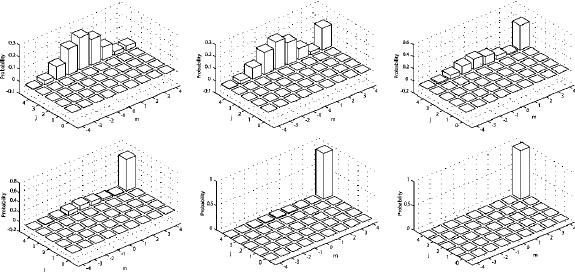
\includegraphics[width=1\textwidth]{images/grover.png}
\caption{Grover's Search}
\end{figure}

\subsection{Optimization: Quantum Annealing}
Classical computing might use what's called "gradient descent": start at a random spot on the surface, look around for a lower spot to walk down to, and repeat until you can't walk downhill anymore. But all too often that gets you stuck in a "local minimum" -- a valley that isn't the very lowest point on the surface.
That's where quantum computing comes in. It lets you cheat a little, giving you some chance to "tunnel" through a ridge to see if there's a lower valley hidden beyond it. This gives you a much better shot at finding the true lowest point -- the optimal solution. We'll see how that works using Quantum annealing.\par\bigskip
\begin{figure}[H]
\centering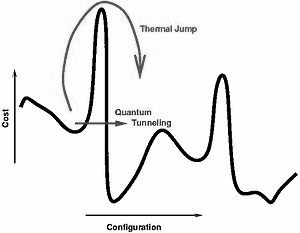
\includegraphics[width=.4\textwidth]{images/anneal.png}
\caption{Quantum annealing}
\end{figure}
Quantum annealing can be compared to simulated annealing, whose "temperature" parameter plays a similar role to Quantum Annealing's tunneling field strength. In simulated annealing, the temperature determines the probability of moving to a state of higher "energy" from a single current state. In quantum annealing, the strength of transverse field determines the quantum-mechanical probability to change the amplitudes of all states in parallel.
The tunneling field is basically a energy term that does not commute with the classical potential energy part. Analytical and numerical evidence suggests that quantum annealing outperforms simulated annealing under certain conditions. Quantum annealing is also used in sampling from high-dimensional probability distributions.
\subsection{Quantum algorithm for linear systems of equations}
Solving a system of linear equations can be thought of as a Matrix inversion problem.The best known classical algorithm to solve matrix inversion takes $O(n^2log(n))$(best proven lower bound) time. Using Quantum algorithms we can perform matrix inversion in logarithmic time complexity of N. This is because using superposition we can find the eigenvectors and eigenvalues of the matrix by eigen decomposition of a matrix in a logarithmic time. This algorithm can be used to improve Least Square fitting , Principal component analysis and support vector machines which is a large margin optimized linear or non-linear classifier.
Due to the prevalence of linear systems in virtually all areas of science and engineering, the quantum algorithm for linear systems of equations has the potential for widespread applicability.\par\bigskip

Other than these basic algorithms that are used in almost all Machine Learning systems there are more complex ones which are applicable for specific systems such ANN, HMM etc. There are Quantum algorithms which can provide exponential speedup for these systems.

\section{Classical learning applied to quantum systems} 
This approach uses classical learning techniques to process large amounts of experimental quantum data in order to characterize an unknown quantum system.\par\bigskip
The ability to experimentally control and prepare increasingly complex quantum systems brings with it a growing need to turn large and noisy data sets into meaningful information. This is a problem that has already been studied extensively in the classical setting, and consequently, many existing machine learning techniques can be naturally adapted to more efficiently address experimentally relevant problems. For example, Bayesian methods and concepts of algorithmic learning can be fruitfully applied to tackle quantum state classification, Hamiltonian learning and the characterization of an unknown unitary transformation.
It has many applications such as 
\begin{itemize}
\item Identifying an accurate model for the dynamics of a quantum system
\item Extracting information on unknown states
\item Learning unknown unitary transformations and measurements
\end{itemize}
As Classical learning on classical data helps us understand the data and the system that produced that data, Classical learning on Quantum data helps us understand Quantum data and the Quantum system that produced that data. 
This is relatively small and current research field. 


\section{Fully quantum machine learning}
In the most general case of quantum machine learning, both the learning device and the system under study, as well as their interaction, are fully quantum. This goes beyond the early quantum computers and requires a much sophisticated Quantum Computer.\par\bigskip
One class of problem that can benefit from the fully quantum approach is that of 'learning' unknown quantum states, processes or measurements, in the sense that one can subsequently reproduce them on another quantum system. For example, one may wish to learn a measurement that discriminates between two coherent states, given not a classical description of the states to be discriminated, but instead a set of example quantum systems prepared in these states. The naive approach would be to first extract a classical description of the states and then implement an ideal discriminating measurement based on this information. This would only require classical learning. However, one can show that a fully quantum approach is strictly superior in this case. (This also relates to work on quantum pattern matching.) The problem of learning unitary transformations can be approached in a similar way.
A fully quantum clustering algorithm is also available - A Quantum Nearest-Centroid Algorithm for k-Means Clustering k-means clustering is a popular machine learning algorithm that structures an unlabelled dataset into k classes. k-means clustering is an NP-hard problem. The complexity arguments on the dependence of m were rigorously confirmed using the QPCA construction for a support vector machine (SVM) algorithm. This can roughly be thought of as a k-means clustering problem with $k=2$. A speedup is obtained due to the classical computation of the required inner products being $O(nm)$.


